%\documentclass{beamer}
\documentclass[10pt]{beamer}
\usepackage{etex}


\setbeamercolor*{frametitle}{bg=white,fg=gray}
\setbeamerfont{frametitle}{series=\mdseries}

\usepackage{xmpmulti}

\usepackage{soul}
\usepackage{cancel}
\usepackage{beamerthemesplit}
%\usepackage{multimedia}
\usepackage{media9}
\usepackage{overpic}
\usepackage{color}
\usepackage{bm}
\usepackage{graphicx} % more modern
%\usepackage{epsfig} % less modern
\usepackage{subfigure}
\usepackage{multirow}
\usepackage{listings}

\usepackage{tcolorbox}

\usepackage{mathtools}


\newlength\fheight
\newlength\fwidth


\usepackage{contour}

%\usepackage{enumitem}

%\usepackage[english]{babel}
%\usepackage[utf8]{inputenc}


\usepackage{tikz}
%\usetikzlibrary{calc}
%\usetkzobj{all}

%\usepackage{pgfplots}
\newlength\figureheight 
\newlength\figurewidth 

\usepackage{xypic}


%\usepackage{pgf,tikz}
%\usepackage{tkz-euclide}
%\usepackage{tkz-graph}
%\usetikzlibrary{calc}
%\usetkzobj{all}



\setbeamertemplate{navigation symbols}{}
\usefonttheme{professionalfonts}
\useoutertheme{split}
\useinnertheme{circles}

\usepackage{extarrows}
\usepackage{amsfonts}
\usepackage{algorithmic}\usepackage{algorithm}\newtheorem{de}{Definition}[section]
\newtheorem{theo}{Theorem}[section]
\newtheorem{prop}{Proposition}[section]
\newtheorem{lem}[theo]{Lemma}
\newcommand{\argmax}{\operatornamewithlimits{argmax~}}
\newcommand{\argmin}{\operatornamewithlimits{argmin~}}
\newcommand{\diag}{\operatorname{diag}}
\newcommand{\sinc}{\operatorname{sinc}}
\newcommand{\comb}{\operatorname{comb}}
\newcommand{\rect}{\operatorname{rect}}
\newcommand{\erf}{\operatorname{erf}}
\newcommand{\diver}{\operatorname{div}}
\newcommand{\sgn}{\operatorname{sign}}
\newcommand{\dom}{\operatorname{dom}}
\newcommand{\trace}{\operatorname{trace}}
\newcommand{\interior}{\operatorname{int}}

\newcommand{\bb}[1]{\boldsymbol{\mathrm{#1}}}

\def\Tr{\top}

\newcommand{\EE}{\mathbb{E}}
\newcommand{\HH}{\mathbb{H}}


\newcommand{\aaa}{\bb{a}}
\newcommand{\eee}{\bb{e}}
\newcommand{\pp}{\bb{p}}
\newcommand{\qq}{\bb{q}}
\newcommand{\uu}{\bb{u}}
\newcommand{\vv}{\bb{v}}
\newcommand{\ww}{\bb{w}}



\newcommand{\xx}{\bb{x}}
\newcommand{\yy}{\bb{y}}
\newcommand{\zz}{\bb{z}}


\newcommand{\ones}{\bb{1}}
\newcommand{\zeros}{\bb{0}}


\newcommand{\Ee}{\bb{E}}


\newcommand{\Pp}{\bb{P}}
\newcommand{\ttt}{\bb{t}}


\newcommand{\RR}{\mathbb{R}}

\newcommand{\Rr}{\bb{R}}

\newcommand{\Aa}{\bb{A}}
\newcommand{\Bb}{\bb{B}}
\newcommand{\Cc}{\bb{C}}
\newcommand{\Xx}{\bb{X}}
\newcommand{\Yy}{\bb{Y}}
\newcommand{\Vv}{\bb{V}}
\newcommand{\Uu}{\bb{U}}
\newcommand{\Dd}{\bb{D}}
\newcommand{\Ii}{\bb{I}}

\newcommand{\Ww}{\bb{W}}
\newcommand{\Ll}{\bb{L}}


\newcommand{\Llambda}{\bb{\Lambda}}
\newcommand{\Pphi}{\bb{\Phi}}
\newcommand{\Ppsi}{\bb{\Psi}}

\newcommand{\Log}{\mathrm{Log}\,}
\renewcommand{\det}{\mathrm{det}\,}


\providecommand{\mycite}[1]{\vskip 0pt plus 1filll{\begin{flushleft}\footnotesize \color{gray}{#1}\end{flushleft} }}


\usetheme{Copenhagen}
\setbeamertemplate{footline}{}
\setbeamertemplate{navigation symbols}{}
\addtobeamertemplate{navigation symbols}{}{%
	\usebeamerfont{footline}%
	\usebeamercolor[fg]{footline}%
	\hspace{1em}%
	\insertframenumber/\inserttotalframenumber
}
\setbeamercovered{invisible}



\title[DLAI]{Deep Learning}
\author[Emanuele Rodol\`a]{{\bf Emanuele Rodol\`a}
\\ \medskip 
}
\date{\today}


\definecolor{red}{rgb}{0.75,0,0}
\definecolor{blue}{rgb}{0,0,0.75}

\definecolor{darkred}{rgb}{0.75,0,0}
\definecolor{darkblue}{rgb}{0,0,0.75}
\definecolor{darkgreen}{rgb}{0,0.75,0}

\newcommand{\resaltar}[1]{{\color{darkblue}#1}}
\newcommand{\redaltar}[1]{{\color{darkred}#1}}
\newcommand{\regaltar}[1]{{\color{darkgreen}#1}}


\newcommand<>{\uncoverubrace}[2]{%
  \onslide#3 \underbrace{ \onslide<1->%
  #1%
  \onslide#3 }_{#2} \onslide<1->%
}
\newcommand<>{\uncoverobrace}[2]{%
  \onslide#3 \overbrace{ \onslide<1->%
  #1%
  \onslide#3 }^{#2} \onslide<1->%
}



\date{}



\newif\ifmovies

\moviestrue


\def\Circlearrowleft{\ensuremath{%
  \rotatebox[origin=c]{180}{$\circlearrowleft$}}}
\def\Circlearrowright{\ensuremath{%
  \rotatebox[origin=c]{180}{$\circlearrowright$}}}
\def\CircleArrowleft{\ensuremath{%
  \reflectbox{\rotatebox[origin=c]{180}{$\circlearrowleft$}}}}
\def\CircleArrowright{\ensuremath{%
  \reflectbox{\rotatebox[origin=c]{180}{$\circlearrowright$}}}}



\usepackage{fontspec}
\setmainfont[Path=../,
 BoldFont={Biancoenero-Bold.ttf},
 ItalicFont={Biancoenero-Italic.ttf},
 BoldItalicFont={Biancoenero-Bold-Italic.ttf}
 ]{Biancoenero-Regular.ttf}
\setmonofont[Path=../]{Biancoenero-Regular.ttf}
\setsansfont[Path=../,
 BoldFont={Biancoenero-Bold.ttf},
 ItalicFont={Biancoenero-Italic.ttf},
 BoldItalicFont={Biancoenero-Bold-Italic.ttf}
 ]{Biancoenero-Regular.ttf}
 


\begin{document}





\frame{
	\begin{center}
		
		\bigskip
		{\Huge 
			\bf Deep Learning \& \\ Applied AI
		}
		
		\bigskip\bigskip
		
		{\Large
		Linear regression, convexity, and gradients
		}
		
		
		\bigskip \medskip \bigskip
		
		{\large 
			
			Emanuele Rodol\`a
			
			\smallskip
			
			{\color{blue}{rodola@di.uniroma1.it}}
		}
		
		\bigskip

  \includegraphics[width=0.14\linewidth]{../sapienza.png}

		
		\bigskip
		\bigskip
		


		\bigskip\bigskip
		\footnotesize 2nd semester a.y. 2025/2026 $\cdot$ March 3, 2026
		
	\end{center}
}




\begin{frame}
\frametitle{A glimpse into neural networks}

In deep learning, we deal with \resaltar{highly parametrized models} called \resaltar{deep neural networks}:

\only<3>{
\begin{center}
		\begin{overpic}
		[trim=0cm 0cm 0cm 0cm,clip,width=0.99\linewidth]{./figures/nn1}
		\end{overpic}
\end{center}}%
\only<4->{
\begin{center}
		\begin{overpic}
		[trim=0cm 0cm 0cm 0cm,clip,width=0.6\linewidth]{./figures/nn1}
		\end{overpic}
\end{center}}%
\only<1-2>{
\begin{center}
		\begin{overpic}
		[trim=0cm 0cm 0cm 0cm,clip,width=0.99\linewidth]{./figures/nn2}
\only<1>{		\put(46,25){\Huge $f_{\bm{\Theta}}$}}
\only<2>{		\put(35,25){\Huge $f_{\bm{\Theta}}(\mathbf{x}) = \mathbf{y}$}}
%\only<2>{    \put(-3,25){\Huge $\mathbf{x}$}}
		\end{overpic}
\end{center}}

\begin{itemize}
\item<4-> Each block has a predefined structure (e.g., a \resaltar{linear map})
%\smallskip

\item<5-> Each block is defined in terms of \resaltar{unknown parameters} $\theta$
%\smallskip

\item<6-> Finding the parameter values is called \resaltar{training}...
%\smallskip

\item<7-> ...which is done by minimizing a function called \resaltar{loss}
%\smallskip

\item<8-> Minimization requires computing gradients, called \resaltar{backpropagation}

\end{itemize}

\mycite{}
\end{frame}




%
%\begin{frame}
%\frametitle{Parametrized models}
%
%The parameters determine the network's behavior and must be \resaltar{solved for}.
%
%\medskip
%
%\begin{center}
%		\begin{overpic}
%		[trim=0cm 0cm 0cm 0cm,clip,width=0.99\linewidth]{./figures/funcs}
%\only<1>{{\put(9,-6.5){$y = {\color{darkred}a}x+{\color{darkred}b}$}}
%{		\put(39,-6.5){$y = {\color{darkred}a}x^2 + {\color{darkred}b}x+{\color{darkred}c}$}}
%{\put(70.5,-6.5){${y = {\color{darkred}a}\sin(x) + {\color{darkred}b}x +{\color{darkred}c}}$}}}%
%\only<2>{
%{\put(4,-6.5){$f_{\color{darkred}a,b}(x) = {\color{darkred}a}x+{\color{darkred}b}$}
%}
%%{		\put(32,-6.5){$g({\color{darkred}a,b,c}) = {\color{darkred}a}x^2 + {\color{darkred}b}x+{\color{darkred}c}$}}
%%{\put(68.5,-6.5){${h({\color{darkred}a,b,c}) = {\color{darkred}a}\sin(x) + {\color{darkred}b}x +{\color{darkred}c}}$}}
%}%
%\only<3->{
%\put(12,-6.5){$f_{\color{darkred}\Theta_f}(x)$}
%\put(8.8,-10.5){${\color{darkred}\Theta_f} \equiv \{{\color{darkred}a,b}\}$}
%\put(47.5,-6.5){$g_{\color{darkred}\Theta_g}(x)$}
%\put(81.5,-6.5){$h_{\color{darkred}\Theta_h}(x)$}
%}
%		\end{overpic}
%\end{center}
%
%\uncover<3->{
%\bigskip\bigskip\medskip\medskip\medskip
%
%Our task is to find the parameters $\Theta$.}
%
%\mycite{}
%\end{frame}



\begin{frame}
\frametitle{Linear regression}

\vspace{-0.1cm}

We start from the simplest non-trivial case for a learning model:

\medskip

\begin{center}
		\begin{overpic}
		[trim=0cm 0cm 0cm 0cm,clip,width=0.3\linewidth]{./figures/linsamples}
		\end{overpic}\hspace{0.5cm}
\uncover<2->{\begin{overpic}
		[trim=0cm 0cm 0cm 0cm,clip,width=0.3\linewidth]{./figures/linfit}
		\end{overpic}}
\end{center}

\vspace{-0.2cm}

\only<2>{
\[ y_i = ax_i + b \]

\smallskip}%
\only<3->{
\[ f_\Theta (x_i) = y_i  \]

\smallskip

\textbf{Model}: linear + bias

\smallskip

\textbf{Parameters}: $\Theta = \{a,b\}$

\smallskip

\textbf{Data}: $n$ pairs $(x_i, y_i)$; the $x_i$ are called the \resaltar{regressors}
}

\uncover<4->{
\medskip\medskip

Given $a$ and $b$, we have a \resaltar{mapping} that gives new output from new input.
}

\mycite{}
\end{frame}





\begin{frame}
\frametitle{Linear regression\uncover<5->{: Loss function}}

\vspace{-0.1cm}

The equations:
%
%\[ y_i = ax_i + b \]
\[ f_\Theta (x_i) = y_i \]
%
must \resaltar{approximately} hold for all $i=1,\dots, n$.

\uncover<2->{
\medskip\medskip

\textbf{Problem:} Choose $a$ and $b$ that minimize the \resaltar{mean squared error (MSE)} between input and predicted output:

\only<2-4>{
\[
\epsilon = \min_{a,b\in\mathbb{R}} \only<2>{\frac{1}{n}} \sum_{i=1}^n  ( y_i - f_\Theta (x_i) )^2
\]}%
\only<5->{
\[
\epsilon = \min_{\Theta} \ell_\Theta ( \{ x_i, y_i \} )
\]}%

\only<2-4>{where $\Theta = \{a,b\}$.

\only<4>{\medskip
When $f_\Theta$ is linear, this is called a \resaltar{least-squares approximation} problem.}}}%
%
\uncover<5->{
\medskip

The error criterion w.r.t. the parameters is also called a \resaltar{loss} function, usually denoted by $\ell$:
%
\[
\ell_\Theta( \{x_i, y_i\} ) = \sum_{i=1}^n  ( y_i - f_\Theta (x_i) )^2
\]}

%\smallskip
\uncover<6->{\textbf{Remark:} We minimize the loss \resaltar{w.r.t. the parameters $\Theta$}, and \textbf{not} w.r.t. the \resaltar{data} $(x_i,y_i)$. Also, the loss is defined on the \resaltar{entire dataset}, not on just one data point.}

\mycite{}
\end{frame}




\begin{frame}
\frametitle{Linear regression}

\bigskip\bigskip

We are considering the following case:

\begin{center}
\hspace{-1.5cm}
		\begin{overpic}
		[trim=0cm 0cm 0cm 0cm,clip,width=0.6\linewidth]{./figures/nn2}
		\put(-10,25){ $\mathbf{x}_i \to$}
		\put(48,25){ $f_{\bm{\Theta}}$}
		\put(99.5,25){$\to \mathbf{y}_i \to {\color{red}\ell_{{\Theta}}(\mathbf{x}_i,\mathbf{y}_i)}$}
		\end{overpic}
\end{center}
%
where $f_{\bm{\Theta}}$ is linear, and $\ell_\Theta$ is quadratic.

\mycite{}
\end{frame}




\begin{frame}
\frametitle{Optimization}

We need to solve the {general} \resaltar{minimization} problem:
%
%\only<1>{
%\[
%\epsilon = \min_{a,b\in\mathbb{R}} \only<2>{\frac{1}{n}} \sum_{i=1}^n  ( y_i - a x_i - b )^2
%\]}%
%\only<2->{
\[
\epsilon = \min_{\Theta} \ell(\Theta)
\]
%}

\uncover<2->{
In particular, we are interested in the \resaltar{minimizer} $\Theta$.
}

\uncover<3->{\bigskip
Finding minimizers for general $\ell$ is an open problem. The research area is broadly called \resaltar{optimization}.

\medskip

In general, the optimization method depends on the properties of $\ell$.
}

\uncover<4->{\bigskip
We will mostly deal with \resaltar{unconstrained} problems.}

\uncover<5->{\bigskip\bigskip
Let's see what optimization problems we can solve \resaltar{easily}!
}

\mycite{}
\end{frame}




\begin{frame}
\frametitle{Convex functions}

\resaltar{Jensen's inequality}:
%
\[
f(\alpha x + (1-\alpha)y) \le \alpha f(x) + (1-\alpha)f(y)
\]
%
for all $x,y$ and $\alpha\in (0,1)$

\medskip

\uncover<2->{
\begin{center}
		\begin{overpic}
		[trim=0cm 0cm 0cm 0cm,clip,width=0.65\linewidth]{./figures/convex}
		\end{overpic}
\end{center}}

\medskip
\uncover<3->{
Let us further assume that $f$ is a \resaltar{differentiable} function, so that we can compute its \resaltar{derivative} $\frac{df}{dx}$ at all points $x$.
}

\medskip
\uncover<4->{
\textbf{Theorem:} the \resaltar{global} minimizer $x$ is where $\frac{df(x)}{dx}=0$.
}

\mycite{}
\end{frame}





\begin{frame}
\frametitle{Convex functions on $\mathbb{R}^n$}

\vspace{-0.15cm}

In deep learning we deal with \resaltar{loss functions} with $n \gg 1$ parameters:
\[
f : \mathbb{R}^n \to \mathbb{R}
\]

\uncover<2->{
The notion of derivative is replaced by the notion of \resaltar{gradient}:
\[
\nabla_\mathbf{x} f(\mathbf{x}) = \begin{pmatrix} \frac{\partial f}{\partial x_1}\\ \vdots \\ \frac{\partial f}{\partial x_n} \end{pmatrix}
\]
which is the vector of \resaltar{partial derivatives} of $f$.
}

\uncover<3->{
\medskip\medskip

Convexity is defined as before:
\[
f(\alpha \mathbf{x} + (1-\alpha)\mathbf{y}) \le \alpha f(\mathbf{x}) + (1-\alpha)f(\mathbf{y})
\]
\uncover<4->{
and we also have the \resaltar{global optimality} condition:
\[
\nabla_\mathbf{x} f(\mathbf{x}) = \mathbf{0} \quad \Longrightarrow \quad f(\mathbf{x}) \le f(\mathbf{y}) ~ \mathrm{for~all~} \mathbf{y}\in\mathbb{R}^n
\]}
}


\mycite{}
\end{frame}



\begin{frame}
\frametitle{The gradient}

The gradient $\nabla_\mathbf{x} f(\mathbf{x})$ encodes the \resaltar{direction} of \resaltar{steepest ascent} of $f$ at point $\mathbf{x}$.\only<2-3>{ In the simple 1D case:}\only<4->{ In the more general case:}

\only<2>{
\begin{center}
		\begin{overpic}
		[trim=0cm 0cm 0cm 0cm,clip,width=0.55\linewidth]{./figures/grad1d}
		\put(52,-4){\footnotesize $x$}
		\put(62,-4){\footnotesize $x+\delta$}
		\put(49,16){\footnotesize $f(x)$}
		\put(67,29){\footnotesize $f(x+\delta)$}
		\end{overpic}
\end{center}}%
\only<3>{
\begin{center}
		\begin{overpic}
		[trim=0cm 0cm 0cm 0cm,clip,width=0.55\linewidth]{./figures/grad1d2}
		\put(52,-4){\footnotesize $x$}
		\put(62,-4){\footnotesize $x+\delta$}
		\put(49,16){\footnotesize $f(x)$}
		\put(67,29){\footnotesize $f(x+\delta)$}
		\put(93,20){\footnotesize $\frac{df(x)}{dx}=\lim\limits_{\delta\to 0} \frac{f(x+\delta)-f(x)}{\delta}$}
		\end{overpic}
\end{center}}%
\only<4->{
\begin{center}
		\begin{overpic}
		[trim=0cm 0cm 0cm 0cm,clip,width=0.60\linewidth]{./figures/grad}
		\end{overpic}
\end{center}}

\uncover<5->{
\smallskip
The \resaltar{length} of the gradient vector encodes its steepness.
}



\mycite{}
\end{frame}



\begin{frame}
\frametitle{Vector lengths}

The \resaltar{Euclidean distance} measures the length of a straight line connecting two points:

\begin{center}
\only<1>{
		\begin{overpic}
		[trim=0cm 0cm 0cm 0cm,clip,width=0.7\linewidth]{./figures/euclidean1.pdf}
	\put(5,20){$\mathbb{R}^2$}
	\put(0,6){$a$}
	\put(36,24){$b$}
		\end{overpic}
}%
\only<2->{
		\begin{overpic}
		[trim=0cm 0cm 0cm 0cm,clip,width=0.7\linewidth]{./figures/euclidean2.pdf}
	\put(5,20){$\mathbb{R}^2$}
	\put(0,6){$a$}
	\put(36,24){$b$}
	%
	\put(49,-4){$(x_a,y_a)$}
	\put(87,25){$(x_b,y_b)$}
	%
	\only<3->{
	\put(65,24){$|x_b-x_a|$}
	\put(95,12){$|y_b-y_a|$}
	}
		\end{overpic}
}
\end{center}

\bigskip
\uncover<4->{
Apply Pythagoras' theorem: $d(a,b) = (   |x_b-x_a|^2 + |y_b-y_a|^2  )^{\frac{1}{2}}$
}

\bigskip
\uncover<5->{
In matrix notation: 

\begin{center}
$d(\mathbf{a},\mathbf{b}) = \| \mathbf{a} - \mathbf{b} \|_2$
\end{center}

  where $\mathbf{a}=\begin{pmatrix}x_a \\ y_a\end{pmatrix}$ and $\mathbf{b}=\begin{pmatrix}x_b \\ y_b\end{pmatrix}$
}

\mycite{}
\end{frame}




\begin{frame}
\frametitle{$L_p$ distance in $\mathbb{R}^k$}

One can generalize to different power coefficients $p\ge 1$:

{
\begin{center}
$ \| \mathbf{x} - \mathbf{y} \|_2 = (   |x_1-y_1|^2 + |x_2-y_2|^2  )^{\frac{1}{2}}$

$\Downarrow$

$ \| \mathbf{x} - \mathbf{y} \|_{\color{red}p} = (   |x_1-y_1|^{\color{red}p} + |x_2-y_2|^{\color{red}p}  )^{\frac{1}{{\color{red}p}}}$
\end{center}
}

\uncover<2->{
As well as generalize from $\mathbb{R}^2$ to $\mathbb{R}^k$:
{
\begin{center}
$\| \mathbf{x} - \mathbf{y} \|_p = ( \sum_{i=1}^k |x_i - y_i|^p )^{\frac{1}{p}}$
\end{center}}
}

\bigskip
\uncover<3->{
This definition gives us the \resaltar{$L_p$ distance} between vectors in $\mathbb{R}^k$.}

\uncover<4->{

\medskip\medskip
The \resaltar{length} (or \resaltar{norm}) of a vector is simply its distance from the origin:

{
\begin{center}
$ \| \mathbf{x} - \mathbf{0} \|_2 =\| \mathbf{x} \|_2= \sqrt{ \sum_{i=1}^k |x_i|^2 }\uncover<5->{=\sqrt{\mathbf{x}^\top\mathbf{x}}}$
\end{center}}
}

\mycite{}
\end{frame}






\begin{frame}
\frametitle{$L_p$ unit balls in $\mathbb{R}^2$}

\begin{center}
  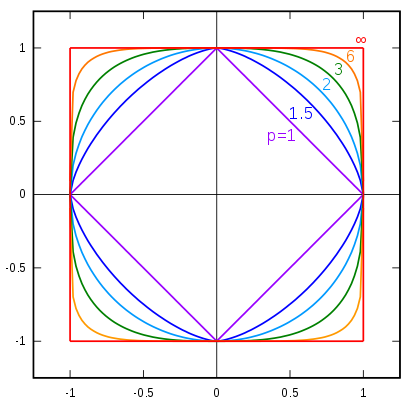
\includegraphics[width=0.63\linewidth]{./figures/norms.png}
\end{center}

\mycite{}
\end{frame}









\begin{frame}
\frametitle{Linear regression: Finding a solution}

\vspace{-0.2cm}

\only<1>{
\[
\min_{a,b\in\mathbb{R}}  \sum_{i=1}^n  ( y_i - a x_i - b )^2
\]}%
\only<2->{
\[
\bm{\Theta}^\ast= \arg\min_{\bm{\Theta}\in\mathbb{R}^2}  \ell(\bm{\Theta})
\]

where $\ell:\mathbb{R}^2\to\mathbb{R}$ is defined as:
%
\[
\ell(a,b) = \sum_{i=1}^n  ( y_i - a x_i - b )^2
\]
}

\uncover<3->{
\smallskip\medskip
A solution is found by setting $\nabla_{\bm{\Theta}} \ell (\bm{\Theta}) = \mathbf{0}$:
}%
\only<3-6>{
%
\begin{align*}
\nabla_{\bm{\Theta}} \sum_{i=1}^n  ( y_i - a x_i - b )^2 &=  \sum_{i=1}^n  \nabla_{\bm{\Theta}} ( y_i - a x_i - b )^2 \\
\uncover<4->{&=  \sum_{i=1}^n  \nabla_{\bm{\Theta}} ( \cancel{y_i^2} + a^2 x_i^2 + b^2 -2a x_i y_i -2by_i +2abx_i )\\}
\only<5>{&= \sum_{i=1}^n \begin{pmatrix} 2ax_i^2 - 2 x_i y_i + 2bx_i \\ 2b - 2y_i + 2ax_i \end{pmatrix}\\}
\only<6->{&=  \begin{pmatrix} \sum_{i=1}^n 2ax_i^2 - 2 x_i y_i + 2bx_i \\ \sum_{i=1}^n 2b - 2y_i + 2ax_i \end{pmatrix}}
\end{align*}
}%
\only<7->{
%
\begin{align*}
\nabla_{\bm{\Theta}} \sum_{i=1}^n  ( y_i - a x_i - b )^2 =\begin{pmatrix} \sum_{i=1}^n 2ax_i^2 - 2 x_i y_i + 2bx_i \\ \sum_{i=1}^n 2b - 2y_i + 2ax_i \end{pmatrix}
\end{align*}
}

\uncover<7->{
\smallskip
We get 2 linear equations in the 2 unknowns $a,b$:% (i.e. the parameters $a$ and $b$):
\[
\begin{pmatrix} \sum_{i=1}^n ax_i^2 + bx_i  -  x_i y_i  \\ \sum_{i=1}^n ax_i + b - y_i  \end{pmatrix} = \begin{pmatrix}0\\0\end{pmatrix}
\]
}


\mycite{}
\end{frame}






\begin{frame}
\frametitle{Linear regression: Matrix notation}

\vspace{-0.1cm}

The learning model of linear regression is \resaltar{linear in the parameters} (while it is \textbf{not} linear in $x$, due to the bias).

\medskip

Therefore, in matrix notation the equations $y_i = a x_i +b$ read:
%
\[
\underbrace{\begin{pmatrix} y_1  \\ y_2  \\ \vdots  \\ y_n \end{pmatrix}}_\mathbf{y} = \underbrace{\begin{pmatrix} x_1 & 1 \\ x_2 & 1 \\ \vdots & \vdots \\ x_n & 1 \end{pmatrix}}_\mathbf{X}  \underbrace{\begin{pmatrix} a \\ b \end{pmatrix}}_{\bm{\theta}}\]
%

\uncover<2->{
\textbf{Remark:} Deep learning frameworks frequently use the alternative expression with the bias encoded separately:
%
\[
\underbrace{\begin{pmatrix} y_1  \\ y_2  \\ \vdots  \\ y_n \end{pmatrix}}_\mathbf{y} = a \underbrace{\begin{pmatrix} x_1 \\ x_2 \\ \vdots  \\ x_n  \end{pmatrix}}_\mathbf{X} + b
\]
}

\mycite{}
\end{frame}





\begin{frame}
\frametitle{Linear regression: Matrix notation}

\bigskip\bigskip
\bigskip

\begin{center} \Large
Familiarize with matrix calculus. 

\vspace{2ex}

When implementing deep nets, we manipulate matrices, vectors, and tensors.

%\uncover<2->{
%\vspace{1cm}

%\textcolor{gray}{(if you need it: brief lecture on matrix manipulation tricks?)}
%}
\end{center}

\mycite{}
\end{frame}





\begin{frame}
\frametitle{Linear regression: Matrix notation}

\[
\underbrace{\begin{pmatrix} y_1  \\ y_2  \\ \vdots  \\ y_n \end{pmatrix}}_\mathbf{y} = \underbrace{\begin{pmatrix} x_1 & 1 \\ x_2 & 1 \\ \vdots & \vdots \\ x_n & 1 \end{pmatrix}}_\mathbf{X}  \underbrace{\begin{pmatrix} a \\ b \end{pmatrix}}_{\bm{\theta}}
\]

This expresses all the equations $y_i = ax_i + b$ at once and makes the linearity w.r.t. $a,b$ evident.

\medskip

The MSE is simply:
%
\[
\ell(\bm{\theta})= \only<1>{\| \mathbf{y} - \mathbf{X} \bm{\theta} \|_2^2}\only<2>{( \mathbf{y} - \mathbf{X} \bm{\theta} )^\top ( \mathbf{y} - \mathbf{X} \bm{\theta} )}\only<3->{\mathbf{y}^\top\mathbf{y} -2 \mathbf{y}^\top \mathbf{X}\bm{\theta} + \bm{\theta}^\top\mathbf{X}^\top \mathbf{X}\bm{\theta}}
\]

\uncover<4->{
Setting $\nabla_{\bm{\theta}} \ell= \mathbf{0}$ we get:
\[
\only<4>{-2 \mathbf{X}^\top \mathbf{y}  + 2 \mathbf{X}^\top \mathbf{X}\bm{\theta} = \mathbf{0}}
\only<5>{\mathbf{X}^\top \mathbf{X}  \bm{\theta} =  \mathbf{X}^\top\mathbf{y}}
\only<6->{\bm{\theta} = (\mathbf{X}^\top \mathbf{X})^{-1} \mathbf{X}^\top\mathbf{y}}
\]}%
\uncover<6->{We get a \resaltar{closed form solution} to our problem.}

\mycite{}
\end{frame}





\begin{frame}
\frametitle{A note on the gradient in matrix form}

%In the previous slide, we computed the gradient of a function $f:\mathbb{R}^2\to\mathbb{R}$, mapping $f:\bm{\theta}\mapsto\epsilon$.

%\medskip
In the previous slide, for the differentiation step:
%
\[
{\mathbf{y}^\top\mathbf{y} -2 \mathbf{y}^\top \mathbf{X}\bm{\theta} + \bm{\theta}^\top\mathbf{X}^\top \mathbf{X}\bm{\theta}} \quad \xRightarrow{\nabla_{\bm{\theta}}}  \quad -2 \mathbf{X}^\top \mathbf{y}  + 2 \mathbf{X}^\top \mathbf{X} \bm{\theta}
\]


what we did is \textbf{exactly equivalent} to the element-by-element computation of slide \#13/20, but we did it directly in matrix form.
 
 \uncover<2->{
 \bigskip
 \underline{Example:} $f(\bm{\theta}) = \bm{\theta}^\top \mathbf{A} \bm{\theta}$
 %
 \begin{align*}
 \nabla_{\bm{\theta}} f(\bm{\theta}) =  
 \only<2>{\nabla_{\bm{\theta}} \begin{pmatrix} \theta_1&\cdots&\theta_n \end{pmatrix} \begin{pmatrix} a_{11}&\cdots&a_{1n} \\\vdots&\ddots&\vdots\\a_{n1}&\cdots&a_{nn}\end{pmatrix}   \begin{pmatrix} \theta_1\\\cdots\\\theta_n \end{pmatrix}}
  \only<3>{\nabla_{\bm{\theta}} \sum_{i=1}^n \sum_{j=1}^n a_{ij}\theta_i\theta_j }
    \only<4>{\begin{pmatrix}\frac{\partial}{\partial \theta_1} \sum_{i=1}^n \sum_{j=1}^n a_{ij}\theta_i\theta_j  \\ \vdots \\\frac{\partial}{\partial \theta_n} \sum_{i=1}^n \sum_{j=1}^n a_{ij}\theta_i\theta_j  \end{pmatrix}}
        \only<5>{\begin{pmatrix} \sum_j a_{1j}\theta_j + \sum_i a_{i1}\theta_i \\ \vdots \\ \sum_j a_{nj}\theta_j + \sum_i a_{in}\theta_i \end{pmatrix}}
                \only<6>{\begin{pmatrix} \sum_i (a_{1i} + a_{i1})\theta_i \\ \vdots \\ \sum_i (a_{ni} + a_{in})\theta_i \end{pmatrix}}
                \only<7->{(\mathbf{A}+\mathbf{A}^\top)\bm{\theta}}
 \end{align*}
 }
 
 \uncover<8->{
 If $\mathbf{A}$ is symmetric (e.g., $\mathbf{A} = \mathbf{X}^\top \mathbf{X}$), then:
 \[
  \nabla_{\bm{\theta}} f(\bm{\theta}) =  2\mathbf{A}\bm{\theta}
 \]
 }

\mycite{}
\end{frame}










\begin{frame}
\frametitle{Linear regression: Higher dimensions}

\vspace{-0.15cm}

Until now we have seen the case where:
%
\[
y_i = ax_i + b ~~~\mathrm{for~} i=1,\dots,n
\]
that is, each data point is one-dimensional (just one number).

\uncover<2->{
\bigskip

In the more general case, the data points $(\mathbf{x}_i,\mathbf{y}_i)$ are vectors in $\mathbb{R}^d$:
%
\[
\mathbf{y}_i = \mathbf{Ax}_i + \mathbf{b} ~~~\mathrm{for~} i=1,\dots,n
\]


\uncover<3->{
\bigskip

Defining the matrices ${\mathbf{X}}=\left(\begin{smallmatrix}|&|&\\\mathbf{x}_1&\mathbf{x}_2&\cdots\\|&|&\\1&1&\end{smallmatrix}\right), \mathbf{Y}=\left(\begin{smallmatrix}|&|&\\\mathbf{y}_1&\mathbf{y}_2&\cdots\\|&|&\end{smallmatrix}\right), \bm{\Theta}=\left(\begin{smallmatrix}\mathbf{A} \\\\ \mathbf{b}^\top\end{smallmatrix}\right)\,,$

\bigskip
we get a closed-form solution to $\nabla_{\bm{\Theta}} \ell(\bm{\Theta})=\mathbf{0}$:
\[
\bm{\Theta} = (\mathbf{X} \mathbf{X}^\top)^{-1} \mathbf{X}\mathbf{Y}^\top
\]}
}

\mycite{}
\end{frame}





\begin{frame}
\frametitle{Wrap-up}

\vspace{-1cm}

\only<1-2>{
\begin{center}
\hspace{-1.5cm}
		\begin{overpic}
		[trim=0cm 0cm 0cm 0cm,clip,width=0.6\linewidth]{./figures/nn2}
		\put(-10,25){ $\mathbf{x}_i \to$}
		\put(48,25){ $f_{\bm{\Theta}}$}
		\put(99.5,25){$\to \mathbf{y}_i \to {\color{red}\ell_{{\Theta}}(\mathbf{x}_i,\mathbf{y}_i)}$}
		\end{overpic}
\end{center}}%
\only<3->{
\begin{center}
\hspace{-1.5cm}
		\begin{overpic}
		[trim=0cm 0cm 0cm 0cm,clip,width=0.6\linewidth]{./figures/nn1}
		\put(-10,25){ $\mathbf{x}_i \to$}
				\put(47,21){\footnotesize $\uparrow$}
		\put(43.5,16.5){\footnotesize linear}
				\put(43.5,12.5){\footnotesize block}
		\put(99.5,25){$\to \mathbf{y}_i \to {\color{red}\ell_{{\Theta}}(\mathbf{x}_i,\mathbf{y}_i)}$}
		\end{overpic}
\end{center}}

Sometimes, the learning model is \resaltar{linear} and the loss is \resaltar{quadratic}.

\smallskip

This case can be solved in closed form.

\uncover<2->{
\bigskip
The more data points $(\mathbf{x}_i,\mathbf{y}_i)$ we have, the better.
}

\uncover<3->{
\bigskip
\begin{itemize}
\item<3-> MLP: Linear blocks alternated with \resaltar{nonlinear} functions

\medskip
\item<4-> \resaltar{Deep linear networks}: Simple sequence of linear blocks
\end{itemize}
}

\mycite{\uncover<4->{Saxe et al, Exact solutions to the nonlinear dynamics of learning in deep linear neural networks, 2013}}
\end{frame}







\begin{frame}
\frametitle{Suggested reading}

For convexity and optimality, read Sections 3.1.1 and 3.1.3 of the book:

\medskip
S. Boyd \& L. Vandenberghe, ``Convex optimization''. Cambridge University Press, 2009

\smallskip
{\footnotesize Public download link: \url{https://web.stanford.edu/~boyd/cvxbook/bv_cvxbook.pdf}}

\mycite{}
\end{frame}




\end{document} 
